%Context
\chapter{背景介绍}
\label{sec-context} %Label for cross-referencing

%%%%%%%%%%%%
\begin{remark} \color{blue}
Suggested length: About half a page each for the Need Statement and Problem Statement (plus figures, if any). Another page or two for the design team.
\vspace{0.1in}

\noindent The Context provides background and motivation for your project. It is an enlarged version of the brief context in your Executive Summary.  
\begin{itemize} \tightlist
\item Who came to you with a proposed project area? 
\item What background or context set the stage for your Needfinding and Benchmarking, activities?
\end{itemize}
\normalcolor \end{remark}
%%%%%%%%%%%%

\section{需求陈述}
\label{sec:need}

%%%%%%%%%%%%
\begin{remark} \color{blue}
This section is the high-level result of your user need-finding. It defines the ``Point of View'' or hypothesis that guides your ongoing work. 
\begin{itemize} \tightlist
\item Who wants or needs your product? Why do they want it? Or, what need does the product area address? 
\item What evidence do you have to substantiate the need? Use citations or other evidence you've gathered.
\end{itemize}
\noindent The remaining text is taken from \cite{Autodesk2008Fall}.
\normalcolor
\end{remark}
%%%%%%%%%%%%

% The design world has changed dramatically in the last decade. The widespread advancement and usage of digital prototyping tools has made it simpler and faster to realize new ideas. At the same time, globalization is requiring designers from remote locations to combine their ideas and make design decisions. 

% With the advancement of computational power and communication speed, digital prototyping tools have made it possible to transmit complex drawings around the world. Most digital tools that promote remote collaboration target the idea-to-conception stage of development. The early ideation stages of engineering design, however, are still more effective when discussed locally. The problems of effective communication and effective decision-making in this setting are still largely unsolved. Internet tools setup the virtual meeting space, yet communication is still not as effective as meeting in the same room. Often meeting participants cannot truly work together as they do face-to-face.

% Wouldn't it be perfect to have a new tool that focused on the interaction aspects of remote collaboration? A tool that made communication effortless, as if the participants were in the same room. Such a tool could increase the ideation potential of remote meetings and make remote brainstorming a reality. 

整体目标:

我们旨在设计出一种实时的远程音视频通信,将两处的信息交流接合,这种设计基于一台有灵敏移动性能且具备基础的环境障碍感知能力的移动机器人。

背景及意义:

随着计算机、互联网技术的飞速发展,人与人、人与事物之间的联系日益密切,人们所接触的范围也逐渐广泛起来,于此同时,所需要的信息流量也会大大增加,传统的传递方式也许并不能很好的起到传递效果。如果让数字化介入其中,便会收获更好的结果。

试想一下,当某一个机构或部门需要向外界介绍他们的相关信息,这些信息会给参观者留下非常重要的印象,如果诸如此类的信息能够具有实时性、全方位性,并且能够充分调动参观者的主观感受,那么这些信息的价值便会大大提升。

通过远程呈现的基本构架,借助移动机器人提供的主观能动性,搭建如此的一个集散控制的参观导航系统,便会具有如上所述的极佳的效果。

当你身处千里之外,通过简单的互联网界面,点击鼠标、敲击键盘,就可以达到参观目的地的效果,而且这种信息的获取是实时动态的,该是一件多么惬意的事情,你一定会对目标地点有一个非常好的主观印象。而且,你还可以随时与那里的工作人员等互动交流,岂不是更加便捷、实用!



\section{问题陈述}
\label{sec:problem}

%%%%%%%%%%%%%%%
\begin{remark} \color{blue}
Here you get more specific about the particular problem that your design vision is addressing.
The remaining text is again taken from \cite{Autodesk2008Fall},
\normalcolor
\end{remark}
%%%%%%%%%%%%%%%

%In order to facilitate remote collaboration in the early design stage, we first break down the problem into the following three areas.

进一步分析目标,我们可以将过程中需要着重注意、解决的难题归纳总结,分成不同的项目部分,以备后续逐步实现预订功能。如下为分类:

\begin{itemize} \tightlist
\item 网络连接搭建的方式

\item 远程操作者的使用界面

\item 机器人上的用户界面

\item 机器人的操控方式

\end{itemize}

% Early ideation is a very social process and requires effective interperson communication. Current teleconferencing tools lack in recreating the level of social dynamics present in face-to-face communication.

% Communication tools are a means with which we transmit ideas to each other. This could be either through speaking, body language, or drawing. The early ideation stage requires a rapid exchange of ideas between all participants in a meeting. How can we utilize communication tools effectively to make such a dialog easier?

% Finally, the brainstorming stage presents a plethora of ideas that need to be archived and categorized for effective decision making. How can we make it easier for meeting participants to save their ideas and retrieve them later? How can information be viewed to facilitate decision making?

对于网络搭建,由于机器人可能部署在任意的网络环境中,因此不能对实现这套
系统的网络有过高的要求与假设。我们的设计目标是部署在机器人上的客户端无
需公网地址段的ip,也无需和使用者处于同一个子网内,只要机器人有一个无线
网络连接,就可以正常工作。

对于使用界面的设定,考虑到跨平台的潜在需求和移动互联网的趋势,应该采用基于网页界面的设计,具体的功能模块后续的设计中会逐渐添加,进而集成到界面中,以达到符合用户使用需求的目标。

机器人的控制方式也是一个非常重要的方面,它直接关系到了机器人的安全性等强制性的因素,而且对于用户体验也是至关重要的。

% \section{Autodesk}
% Since 1982, Autodesk has delivered 2D and 3D visualization tools for clients in manufacturing and design. Some products include the drafting program AutoCAD, digital prototyping software Inventor, and 3D modeler Maya. The company focuses on enhancing the design process by allowing the customer to experience their design through software.

%%%%%%%%%%%%%%%%%%%%%%%%%%%%%%%%%%%%%%%%%%%%%%%%%%

\section{组员介绍}
\label{sec:team}

%%%%%%%%%%%%%%%%%%%
\begin{remark} \color{blue}
See other recent reports for other ways of introducing the team. To the extent that the characteristics of the team influence the project direction, this is of interest to the reader.
\end{remark} \normalcolor
%%%%%%%%%%%%%%%%%%%

% Team \pmt, was assembled by the ME310 teaching staff, based on the outcome of Myers-Briggs personality tests (see Table \ref{wildeprefs}) and a desire to create teams with a diversity of interests and backgrounds. There is some evidence that such diversity enhances team creativity \cite{Wilde97} \cite{Wilde07}, even if it creates additional challenges for team management.

% Example table. It gets a caption and reference label.
% The tabular formatting is a bit painful...  An alternative is to use Word
% and insert the PDF printout as for a figure. There are also Word-to-Latex converters.
% \begin{table}
%   \begin{tabular}{| p{14mm} | p{20mm} | p{20mm} | p{22mm} | p{20mm} | p{12mm} |} 
%   \hline
% Score & Extroverted-Introverted (E-I) & Intuition-Sensing (N-S) & Feeling-Thinking (F-T) & Perception-Judging (P-J) & Overall \\
% People & & & & &\\
% \hline
% Eric & +6 & +6 & -6 & +12 & ENTP \\
% Azin & -18 & +30 & -30 & +18 & INTP \\
% Patrick & +6 & +18 & -18 & +6 & ENTP \\
% Salil & -18 & +30 & -30 & +18 & INTP \\
% \hline
% \end{tabular}
% \caption{Team preferences scores using the method of Wilde \cite{Wilde07}. }
%         \label{wildeprefs}  %Tag for referring to table
% \end{table}

% \begin{framed}
% \noindent 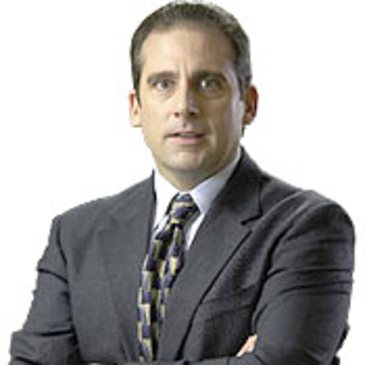
\includegraphics[width=50mm]{Figures/Ch2/Scott}
% \parbox[b]{0.6\textwidth}{Michael Scott\\
% Status: M.E. Graduate Student\\
% Contact: mscott@me310.stanford.edu\\
% Skills: mechatronics, welding, CNC machining\\
% Computing: Solid Works, Matlab, basic C programming, Flash, Dreamweaver\\
% }

% Born in Paris and raised in New Jersey, I attended Columbia University. For graduate school, I decided to trade in the hustle and bustle of New York City for the sunshine of Palo Alto, and so far I have not been disappointed (though New York will always be dear to my heart). My interests include mechatronics, design (including medical devices), football, tennis, pick-up games, tail-gating, Entourage, South Park.
% \end{framed}

\begin{framed}
\noindent 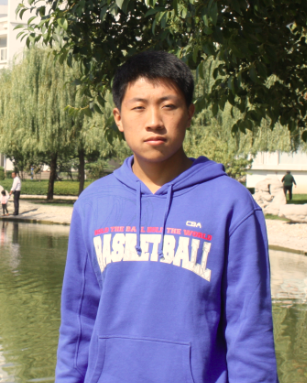
\includegraphics[width=50mm]{Figures/context.pic.png}
\parbox[b]{0.6\textwidth}{王照栋\\
现况:中国科学技术大学,自动化系,10级本科生\\
邮件:wangzd@mail.ustc.edu.cn\\
技能:基础机械结构设计,自动控制\\
编程:C语言编程,初步C++面向对象编程,matlab\\
}

来自山东,2010年考入中科大信息学院,后就读于自动化系。喜欢设计,并且具有一定的动手能力,2012年暑期与同学组队参加过Robogame机器人大赛,并最终获最佳技术奖单项奖。课余时间比较喜欢参与一些运动以及益智类的活动,热爱乒乓球、篮球、羽毛球、游泳等运动,对魔方速拧还原有一定的研究。
\end{framed}

\begin{framed}
\noindent
%\parbox[b]{0.6\textwidth}
{贾肇聪\\
现况:中国科学技术大学10级少年班学院\\
}
自由软件爱好者,在本项目中负责linux服务器的管理和网络维护。
\end{framed}

%%%%%%%%%%%%%%%%%%MORE LATEX EXAMPLES%%%%%%%%%%%%%%
% Let's test some in-situ glossary items. The idea is to insert these kinds of definitions anywhere,
% as they occur to you while incrementally working on the documentation.
%See main file for notes about how to convert the ".glo" file to a glossary section.

% \glossary {paper weight}{ the combined weight of all paper products (paper, cardboard, crepe paper, paper tape) in the vehicle.}
% \glossary {non-paper weight}{ the combined weight of all non paper items (e.g. metal pins, teflon tape, screws). Non-paper weight is severely restricted in ME310 Paper Bike exercises.}
% \glossary {papier m\^{a}ch\`{e} }{a composition of shredded paper glued together with library paste}
% \glossary {particle board} {a product made of compressed wood chips and resin, often sold in 4 ft x 8 ft sheets. Particle board is not considered a paper product.}
% \glossary {sound deadener board} {a product made of compressed cardboard fibers and resin, often sold in 4 ft x 8 ft sheets. Sound deadener board is not considered a paper product.}

\begin{remark} \color{blue}
\section*{Experiments with tables in Latex}

Here is a centered tabular form that is 3/5 of the current text width and has a horizontal line but no
vertical lines:

 \begin{center}  % put inside center environment
  \begin{tabular*}{0.6 \textwidth}%
     {@{\extracolsep{\fill}}cccr}
  \multicolumn{3}{c}{a label spanning 3 merged cells} & label 4  \\
  \hline  % put a line under headers
  item 1a  & item 2a  & item 3a  & item 4a  \\
  item 1b  & item 2c  & item 3c  & item 4c  \\
  \end{tabular*}
  \end{center}

\noindent For anything more complicated than the examples in this section, it may be easiest to do the table in MS Word or OpenOffice, create a pdf and include the pdf in a table environment, as done in Table \ref{tab:physical-requirements}. Because pdf files have scalable fonts, the print resolution will be good.

\end{remark}\normalcolor

